\documentclass[a4paper,11pt]{article}
\usepackage[a4paper,margin=2.5cm]{geometry}
\usepackage{amsmath,amssymb,graphicx,xcolor,booktabs}
\usepackage[colorlinks=true,linkcolor=blue!50!black,citecolor=blue!50!black]{hyperref}
\newcommand{\ndof}{n_\mathrm{dof}}
\newcommand{\dd}{\mathrm{d}}
\renewcommand{\thesection}{2}
\setcounter{section}{2}
\renewcommand{\thesubsection}{2.\arabic{subsection}}
\setcounter{subsection}{4}
\renewcommand{\theequation}{2.\arabic{equation}}
\renewcommand{\thefigure}{2.\arabic{figure}}
\title{Paper 1 --- proposed revision of section 2.5\\[0.3ex]
\large ``Requiring at least $k$ of $N$ planes''}
\author{Draft for discussion, 13 October 2026}
\date{}
\begin{document}
\maketitle

\noindent\textit{Equation numbers are local to this note. References to other sections
(2.2, 2.3, 2.6, 4) are to the current paper. The text below would replace the present
section 2.5 entirely; notes for the authors follow at the end.}

\subsection{Requiring at least $k$ of $N$ planes}\label{sec:kofn}

\paragraph{Why sets of planes.} A real detector is not fully efficient, and a track finder
that required a hit on every plane would lose every track with a missing hit. Track finders
therefore accept candidates with hits on \emph{at least} $k$ of the $N$ planes, five of six
for example. Any such algorithm must also accept the noise combinations that pass on a subset
of the planes. We therefore extend the counting of section~2.2 from one set of planes to all
the sets that the algorithm accepts.

\paragraph{Candidates.} Let $S$ be a set of planes with $|S|\ge k$. A \emph{candidate on $S$}
is a choice of one hit on each plane of $S$, nothing being required of the planes outside
$S$. It is fitted to the track model with the planes of $S$ only, with
$\ndof(S)=2|S|-4$ degrees of freedom, and it is \emph{accepted} if
\begin{equation}
  \chi^2_S < c_S \quad\text{and}\quad \hat\theta_S\in\Theta ,
  \label{eq:accept}
\end{equation}
where $\hat\theta_S$ are the fitted parameters. Each set has its own cut $c_S$, chosen at the
same efficiency for real tracks as for the full set. With our one-sided $3\sigma$ choice the
cut depends only on $\ndof(S)$: for five of six planes, $c=25.36$ for the full set
($\ndof=8$) and $c=21.74$ for each of the six five-plane sets ($\ndof=6$).

\paragraph{The expected number of accepted candidates.} We define $E(\ge k)$ as the expected
number of accepted candidates, summed over all sets of at least $k$ planes. A candidate on $S$
is accepted with probability $P_S$, the probability of section~2.3 computed for the planes of
$S$ alone (their depths, sizes and resolutions), and there are $\prod_{i\in S}n_i$ candidates
on $S$. By linearity of expectation, as in eq.~(2.1),
\begin{equation}
  E(\ge k) \;=\; \sum_{S:\,|S|\ge k} E_S ,\qquad E_S \;=\; P_S\prod_{i\in S} n_i .
  \label{eq:kofn}
\end{equation}
For at least five of six planes the sum has seven terms:
\begin{equation}
  E(\ge 5) \;=\; P_{123456}\;n_1n_2n_3n_4n_5n_6 \;+\; \sum_{j=1}^{6}\,P_{\bar\jmath}\prod_{i\ne j} n_i ,
  \label{eq:5of6}
\end{equation}
where $\bar\jmath$ denotes the five planes other than $j$. Note that a candidate on five planes
is counted whether or not the sixth plane happens to have a hit near the track; this is what an
algorithm accepting five of six planes does.

\begin{figure}[htbp]
  \centering
  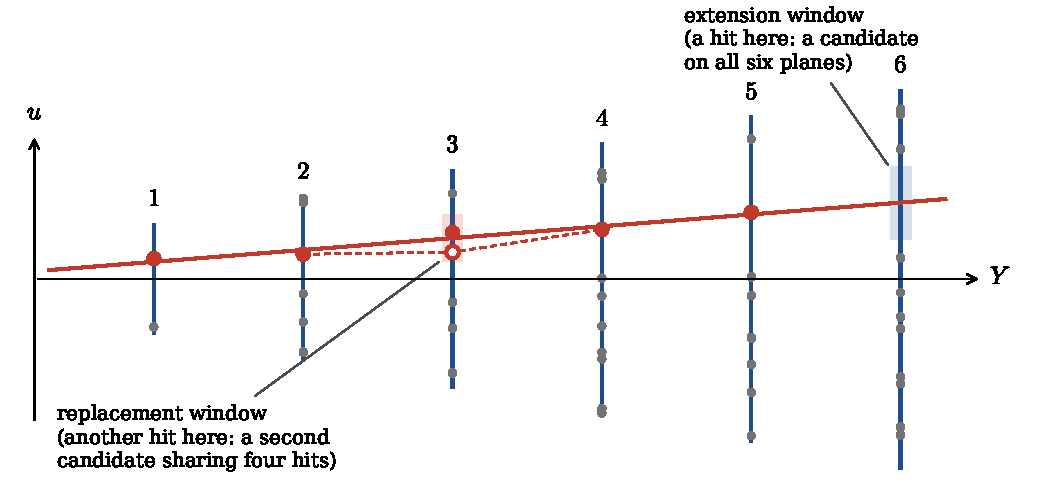
\includegraphics[width=0.9\textwidth]{kofn_sketch}
  \caption{Candidates that share hits, shown in one view and not to scale. A candidate on
  planes 1--5 (filled red points) is accepted. The fit to planes 1, 2, 4 and 5 predicts where
  its hit on plane 3 must lie: any other hit in this \emph{replacement window} (open point)
  forms a second accepted candidate on the same planes, sharing four hits with the first. The
  fit to planes 1--5 predicts plane 6: a hit in this \emph{extension window} forms an accepted
  candidate on all six planes, which contains the first one.}
  \label{fig:windows}
\end{figure}

\paragraph{Windows.} Two accepted candidates can share hits, and the size of the overlap is
governed by a single quantity, the number of hits expected in a \emph{window}
(figure~\ref{fig:windows}). Take an accepted candidate on $S$ and one of its planes, $i$. The
fit to the other planes of $S$ predicts the position $(\hat u_i,\hat v_i)$ of the track on plane
$i$, with variances $V_{u,i}$ and $V_{v,i}$, and has its own $\chi^2_{S\setminus i}$. For a
linear track model the $\chi^2$ of the full set separates exactly into
\begin{equation}
  \chi^2_S \;=\; \chi^2_{S\setminus i} \;+\; \frac{(u_i-\hat u_i)^2}{\sigma_{u,i}^2+V_{u,i}}
  \;+\; \frac{(v_i-\hat v_i)^2}{\sigma_{v,i}^2+V_{v,i}} .
  \label{eq:split}
\end{equation}
Any hit $(u,v)$ on plane $i$ therefore forms an accepted candidate together with the other
hits of $S$ if it lies inside the ellipse in which the last two terms add up to less than
$b_i=c_S-\chi^2_{S\setminus i}$, the part of the $\chi^2$ budget not used by the other planes.
The area of this ellipse is $\pi b_i\sqrt{(\sigma_{u,i}^2+V_{u,i})(\sigma_{v,i}^2+V_{v,i})}$.

The budget $b_i$ varies from candidate to candidate, and its mean is simple. In the whitened
space of section~2.3 the accepted noise combinations fill the $\ndof$-dimensional $\chi^2$
sphere of radius $\sqrt{c_S}$ uniformly, and eq.~\eqref{eq:split} splits the squared distance
from the centre into two coordinates for plane $i$ and $\ndof-2$ for the rest. For a uniformly
filled sphere each coordinate carries on average $c_S/(\ndof+2)$, so the mean of
$\chi^2_{S\setminus i}$ is $c_S(\ndof-2)/(\ndof+2)$ and
\begin{equation}
  \langle b_i\rangle \;=\; \frac{4\,c_S}{\ndof+2} ,
  \label{eq:budget}
\end{equation}
which is $c_S/2$ for $\ndof=6$.

\paragraph{The window occupancy.} The expected number of \emph{other} noise hits in the
replacement window of plane $i$ is its area times the density of the other hits,
\begin{equation}
  \eta_i \;=\; \frac{n_i-1}{A_i}\;\pi\,\langle b_i\rangle\,
  \sqrt{(\sigma_{u,i}^2+V_{u,i})(\sigma_{v,i}^2+V_{v,i})} ,
  \label{eq:eta_i}
\end{equation}
and the \emph{window occupancy} of the candidate is the sum over its planes,
\begin{equation}
  \eta \;=\; \sum_{i\in S}\eta_i .
  \label{eq:eta}
\end{equation}
It is the expected number of other accepted candidates on the same planes that share all but
one hit with the given one. In the same way, for a plane $j$ outside $S$ crossed by the
track, the expected number of hits in the extension window is
\begin{equation}
  \mu_j \;=\; \frac{n_j}{A_j}\;\pi\,\langle b_j\rangle\,\sqrt{(\sigma_{u,j}^2+V_{u,j})(\sigma_{v,j}^2+V_{v,j})},
  \qquad \langle b_j\rangle = c_{S\cup j}-\frac{\ndof(S)}{\ndof(S)+2}\,c_S ,
  \label{eq:mu}
\end{equation}
with $V_{u,j}$, $V_{v,j}$ now the variances of the position predicted on plane $j$ by the fit to
all of $S$.

\paragraph{Why the sets with fewest planes dominate.} Every accepted candidate on $S\cup j$
contains a candidate on $S$, and it is accepted when a hit falls in the extension window of
plane $j$. Therefore, approximately,
\begin{equation}
  E_{S\cup j} \;\simeq\; \mu_j\,E_S ,
  \label{eq:ratio}
\end{equation}
for the tracks of $S$ that cross plane $j$. Each additional plane multiplies the expected number
by the probability that it contains a compatible hit. When the windows are nearly empty, as they
must be for tracking to work at all, $\mu_j\ll1$ and the terms with exactly $k$ planes dominate
the sum~\eqref{eq:kofn}, by a factor $1/\mu$. In the example of section~2.6, at
$10^{-3}$~hits/mm$^2$, $\mu_6=6.0\times10^{-4}$ for the planes 1--5 and plane 6, and
eq.~\eqref{eq:ratio} gives $E_{123456}\simeq 6.0\times10^{-4}\times3.2\times10^{-6}
=1.9\times10^{-9}$, as computed directly from eq.~\eqref{eq:kofn}.

\paragraph{From candidates to distinct fake tracks.} $E(\ge k)$ counts candidates, and the
same fake can appear as several of them, in two ways. (i)~Two candidates on the same planes
share all but one hit (the replacement window). (ii)~A candidate on $S\cup j$ contains
candidates on $S$ (the extension window). A reconstruction algorithm reports such overlapping
candidates as one track. We count as one \emph{distinct fake} each group of accepted candidates
connected by sharing at least $k-1$ hits; an algorithm cannot report fewer distinct fakes than
groups without losing real tracks in the same configurations.

Overlaps of type (ii) are of relative size $\mu$, already small whenever the sets of $k$ planes
dominate. For type (i), each accepted candidate has on average $\eta$ partners. Each pair is
seen from both of its candidates, so when overlaps are rare the number of groups is the number
of candidates minus the number of pairs, $E(\ge k)(1-\eta/2)$. We find that
\begin{equation}
  E_\mathrm{distinct} \;\simeq\; e^{-\eta/2}\,E(\ge k)
  \label{eq:distinct}
\end{equation}
describes the counted number of distinct fakes within a few per cent up to $\eta\approx2$
(section~4), with $\eta$ averaged over the accepted candidates.

\paragraph{Summary.} The lower limit on the number of distinct fake tracks for an algorithm
that accepts at least $k$ of $N$ planes is $E_\mathrm{distinct}$ of eq.~\eqref{eq:distinct},
with $E(\ge k)$ from eq.~\eqref{eq:kofn}. In the regime where tracking is possible the windows
are nearly empty, $\eta\ll1$, and the two coincide: in the example of section~2.6 the
five-plane candidates have $\eta\approx3\times10^{-3}$, so $E_\mathrm{distinct}$ and $E(\ge5)$
differ by 0.15\%. Since $\eta$ grows linearly with the density, it is still only about
$0.02$ at the density where one fake per event is expected ($7.6\times10^{-3}$ hits/mm$^2$),
so the correction remains small wherever the limit matters.

\vspace{2ex}\hrule\vspace{2ex}
\section*{Notes for the authors}

\begin{enumerate}
\item \textbf{What is new compared with the present section 2.5.}
  \begin{itemize}
  \item A definition of a candidate (a set of planes plus one hit on each) and of its
    acceptance, eq.~\eqref{eq:accept}, before $E(\ge k)$ is introduced; $E(\ge k)$ is then
    defined in words as well as by the formula, and written out term by term for five of six
    planes, eq.~\eqref{eq:5of6}.
  \item The windows are derived from the exact $\chi^2$ split of eq.~\eqref{eq:split}, with a
    figure, rather than stated.
  \item The extension window and eq.~\eqref{eq:ratio} explain \emph{why} the terms with the
    fewest planes dominate, with a numerical check against section 2.6.
  \item The distinct-fake count is defined explicitly (groups sharing at least $k-1$ hits,
    which is what the validation of section 4 counts), and the origin of $1-\eta/2$ is
    explained.
  \end{itemize}

\item \textbf{One correction.} The present eq.~(2.8) uses $c/2$ for the mean budget. The
  exact mean for a uniformly filled $\chi^2$ sphere is $4c/(\ndof+2)$, eq.~\eqref{eq:budget}.
  It is $c/2$ for $\ndof=6$, so nothing changes for the five-plane sets, which dominate; for the
  six-plane set ($\ndof=8$) it is $0.4c$ instead of $0.5c$. The validation counts $\eta$ hit by
  hit with the exact budget, so its results are unaffected.

\item \textbf{The lower-limit statement.} Strictly, the lower limit is on distinct fakes,
  $e^{-\eta/2}E(\ge k)$, not on $E(\ge k)$. The difference is negligible in practice (0.15\% in
  the example), but section 2.2 and the conclusions should say ``the expected number of distinct
  fakes'' once the $k$-of-$N$ case is in. I would add one sentence to section 2.2 pointing
  forward to this.

\item \textbf{Numbers.} The values $\eta\approx3\times10^{-3}$ and $\mu_6=6.0\times10^{-4}$ are
  computed for the example of section 2.6 at $10^{-3}$ hits/mm$^2$ (all six five-plane sets have
  $\eta$ between $3.0$ and $3.3\times10^{-3}$). The check of eq.~\eqref{eq:ratio} works for the
  set 1--5 with plane 6 added. For sets missing an inner plane it needs the fraction of tracks
  that cross the missing plane (in the projective tower, many tracks through planes 2--6 miss
  the small plane 1), which is why the text says ``for the tracks of $S$ that cross plane $j$''.

\item \textbf{Possible further simplification.} If the section still feels heavy, the
  extension-window paragraph (eqs.~\eqref{eq:mu}--\eqref{eq:ratio}) could move to the numerical
  example, keeping here only the replacement window and $\eta$. I would keep it here: it is the
  shortest explanation of why five-plane sets dominate, which is the most striking result of
  the example.

\item \textbf{The figure} is a schematic in one view, deliberately not to scale (real windows
  are a few resolutions wide on planes hundreds of millimetres across). It could go in the
  paper as is, or be merged with figure 1 as a second panel.
\end{enumerate}

\end{document}
